\documentclass[11pt, twoside, pdftex]{article}

% This includes all the settings that we should use for the document
\newcommand{\PDFTitle}{Using ROS* on DE-Series Boards}
\newcommand{\commonPath}{../../Common}
\newcommand{\datePublished}{Mar 2022}

\newcommand{\versnum}{21.1} %version number quartus/AMP
\newcommand{\quartusname}{Quartus\textsuperscript{\textregistered} Prime}	
\newcommand{\textBar}{For \quartusname{} \versnum{}}
\newcommand{\thisyear}{2022 } %for copyright
\newcommand{\company}{FPGAcademy.org}
\newcommand{\longteamname}{FPGAcademy.org}
\newcommand{\teamname}{FPGAcademy}
\newcommand{\website}{FPGAcademy.org}

\newcommand{\productAcronym}{AMP}
\newcommand{\productNameShort}{Monitor Program}

\newcommand{\productNameMedTM}{Monitor Program}
\newcommand{\productNameMed}{Monitor Program}

%\newcommand{\headerLogoFilePath}[1]{#1/FPGAcademy.png}



\setlength\topmargin{-0.25in}
\setlength\headheight{0in}
\setlength\headsep{0.35in}
\setlength\textheight{8.5in}
\setlength\textwidth{7in}
\setlength\oddsidemargin{-0.25in}
\setlength\evensidemargin{-0.25in}
\setlength\parindent{0.25in}
\setlength\parskip{0in} 

\pdfpagewidth 8.5in
\pdfpageheight 11in

% listings is a package that supports encapsulating source code in LaTeX conveniently

\usepackage{listings}
% add support for graphics
\usepackage{graphicx}
\usepackage[usenames, dvipsnames]{color}

\def\expandparam\lstinputlisting[#1]#2{\edef\tmp{\noexpand\lstinputlisting[#1]{#2}}\tmp}

\widowpenalty 10000
\clubpenalty 10000

%%%%%%%%%%%%%%%%%%%% Source Code Formatting %%%%%%%%%%%%%%%%%%%%
\definecolor{globalCommentColour}{rgb}{0.588,0.588,0.588}

%%%%%%%%%%%%%%%%%%%%%%%%%%%%%%%%%%%%%%%%%%%%%%%%%%%%
% Defining a NiosII ASM highlighter for lstlisting
\lstdefinelanguage[NiosII]{Assembler} {
 	morekeywords={add, addi, and, andhi, andi, beq, bge, bgeu, bgt, bgtu, ble,  bleu, blt, bltu, bne, br, break,% 
 	bret, call, callr, cmpeq, cmpeqi, cmpge, cmpgei, cmpgeu, cmpgeui, cmpgt, cmpgti, cmpgtu, cmpgtui, cmple,%
 	cmplei, cmpleu, cmpleui, cmplt, cmplti, cmpltu, cmpltui, cmpne, cmpnei, custom, div, divu, eret, flushd,%
 	flushda, flushi, flushp, initd, initda, initi, jmp, jmpi, ldb, ldbio, ldbu, ldbuio, ldh, ldhio, ldhu, ldhuio,%
 	ldw, ldwio, mov, movhi, movi, movia, movui, mul, muli, mulxss, mulxsu, mulxuu, nextpc, nop, nor, or, orhi, ori,%
 	rdctl, rdprs, ret, rol, roli, ror, sll, slli, sra, srai, srl, srli, stb, stbio, sth, sthio, stw, stwio,%
 	sub, subi, sync, trap, wrctl, wrtcl, wrprs, xor, xori, xorhi, xori},% 	
 	morekeywords=[2]{.abort, .ABORT, .align, .app-file, .ascii, .asciz, .balign, .byte, .comm, .data, .def,%
 	.desc, .dim, .double, .eject, .else, .end, .endef, .endif, .equ, .equiv, .err, .extern, .file, .fill, .float,%
 	.global, .globl, .hword, .ident, .if, .include, .int, .irp, .irpc, .lcomm, .lflags, .line, .linkonce, .ln,%
 	.list, .long, .macro, .mri, .nolist, .octa, .org, .p2align, .psize, .quad, .rept, .sbttl, .scl, .section,%
 	.set, .short, .single, .size, .sleb128, .skip, .space, .stadb, .stabn, .stabs, .string, .symver, .tag,%
 	.text, .title, .type, .val, .uleb128, .word},% 	
 	morekeywords=[3]{et, bt, gp, sp, fp, ea, sstatus, ra, pc, status, estatus, bstatus, ienable, ipending, cpuid,%
 	exception, pteaddr, tlbacc, tlbmisc, eccinj, badaddr, config, mpubase, mpuacc},% 	
 	sensitive=t,%
 	alsoletter=.,%
	morestring=[b]",%
 	morecomment=[s]{/*}{*/},%
 	morecomment=[l]\#,%
   }[keywords,comments,strings]
   
   %% NOTE: morekeywords=[2] are GNU directives.
   
   \definecolor{niosInstructionColour}{rgb}{0.000,0.608,0.000}
   \definecolor{niosDirectiveColour}{rgb}{0.000,0.000,0.902}
   \definecolor{niosSpecialRegColour}{rgb}{0.000,0.000,0.000}
   \definecolor{niosStringColour}{rgb}{0.808,0.482,0.000}
   
   %% NOTE: To make bold use: =\bfseries\color{<colour>}
   \lstdefinestyle{defaultNiosStyle} {
   language=[NiosII]{Assembler},
   stringstyle=\color{niosStringColour},
   keywordstyle=\color{niosInstructionColour},
   keywordstyle=[2]\color{niosDirectiveColour},
   keywordstyle=[3]\itshape\color{niosSpecialRegColour}
   }
%%%%%%%%%%%%%%%%%%%%%%%%%%%%%%%%%%%%%%%%%%%%%%%%%%%%

%%%%%%%%%%%%%%%%%%%%%%%%%%%%%%%%%%%%%%%%%%%%%%%%%%%%
% Defining a ArmA9 ASM highlighter for lstlisting
\lstdefinelanguage[ArmA9]{Assembler} {
 	morekeywords={ADC, ADD, ADDS, AND, ANDS, B, BAL, BEQ, BGE, BGT, BL, BLT, BIC, BKPT, BLX, BNE, BX, CDP, CLZ, CMN, CMP, EOR,%
 	EORS, LDC, LDM, LDR, LDRB, LDRBT, LDRH, LDRSB, LDRSH, LDRT, LSL, MCR, MLA, MOV, MOVW, MOVT, MRC, MRS, MSR, MUL, MVN, ORR, PLD,%
 	ROR, RSB, RSC, SBC, SMLAL, SMULL, STC, STM, STR, STRB, STRBT, STRH, STRT, SUB, SUBS, SWI, SWP, SWPB, TEQ, UMLAL,
 	PUSH, POP, MOVS, RORS, LSR},%
 	morekeywords=[2]{.abort, .ABORT, .align, .app-file, .ascii, .asciz, .balign, .byte, .comm, .data, .def,%
 	.desc, .dim, .double, .eject, .else, .end, .endef, .endif, .equ, .equiv, .err, .extern, .file, .fill, .float,%
 	.global, .globl, .hword, .ident, .if, .include, .int, .irp, .irpc, .lcomm, .lflags, .line, .linkonce, .ln,%
 	.list, .long, .macro, .mri, .nolist, .octa, .org, .p2align, .psize, .quad, .rept, .sbttl, .scl, .section,%
 	.set, .short, .single, .size, .sleb128, .skip, .space, .stadb, .stabn, .stabs, .string, .symver, .tag,%
 	.text, .title, .type, .val, .vectors, .uleb128, .word},%
 	morekeywords=[3]{SP, PC, MIDR, CTR, TCMTR, TLBTR, MPIDR, ID_PFR0, ID_PFR1, ID_DFR0, ID_MMFR0, ID_MMFR1, ID_MMFR2,%
 	ID_MMFR3, ID_ISAR0, ID_ISAR1, ID_ISAR2, ID_ISAR3, ID_ISAR4, CCSIDR, CLIDR, AIDR, CSSELR, TTBR0, TTRB1, TTBR2, DACR,%
 	DFSR, IFSR, ADFSR, AIFSR, DFAAR, IFAR, ICIALLUIS, BPIALLIS, PAR, ICIALLU, ICIMVAU, BPIALL, DCIMVAC, DCISW, V2PCWPR,%
 	DCCVAC, DCCSW, DDIMVAC, DCISW, TLBALLIS, TLBIMVAIS, TLBIASIDIS, TLBIMVAAIS, TLBIALL, TLBIMVA, TLBIASID, TLBIMVAA,%
 	PMCR, PMCNTENSET, PMCNTENCLR, PMOVSR, PMSWINC, PMSELR, PMXEVTYPER, PMXEVCNTR, PMUSERENR, PMINTENSET, PMINTENCLR,%
 	PRRR, NRRR, PLEIDR, PLEASR, PLEFSR, PLEUAR, PLEPCR, VBAR, MVBAR, ISR, FCSEIDR, CONTEXTIDR, TPIDRURW, TPIDRURO, TPIDRPRW},%
 	sensitive=f,%
 	alsoletter=.,%
	morestring=[b]",%
 	morecomment=[s]{/*}{*/},%
 	morecomment=[l]{//},%
   }[keywords,comments,strings]
   
   %% NOTE: morekeywords=[2] are GNU directives.
   
   \definecolor{armInstructionColour}{rgb}{0.000,0.608,0.000}
   \definecolor{armDirectiveColour}{rgb}{0.000,0.000,0.902}
   \definecolor{armSpecialRegColour}{rgb}{0.000,0.000,0.000}
   \definecolor{armStringColour}{rgb}{0.808,0.482,0.000}
   
   \lstdefinestyle{defaultArmStyle} {
   language=[ArmA9]{Assembler},
   stringstyle=\color{armStringColour},
   keywordstyle=\color{armInstructionColour},
   keywordstyle=[2]\color{armDirectiveColour},
   keywordstyle=[3]\itshape\color{armSpecialRegColour}
   }
%%%%%%%%%%%%%%%%%%%%%%%%%%%%%%%%%%%%%%%%%%%%%%%%%%%%

%%%%%%%%%%%%%%%%%%%%%%%%%%%%%%%%%%%%%%%%%%%%%%%%%%%%
% Defining style for the verilog.

\definecolor{verilogCommentColour}{rgb}{0.000,0.502,0.000}

\lstdefinestyle{defaultVerilogStyle} {
language={Verilog},
keywordstyle=\color{blue},
commentstyle=\color{verilogCommentColour}
}
%%%%%%%%%%%%%%%%%%%%%%%%%%%%%%%%%%%%%%%%%%%%%%%%%%%%

%%%%%%%%%%%%%%%%%%%%%%%%%%%%%%%%%%%%%%%%%%%%%%%%%%%%
% Defining style for the vhdl.
\lstdefinestyle{defaultVHDLStyle} {
language={VHDL},
keywordstyle=\color{blue},
commentstyle=\color{verilogCommentColour}
}
%%%%%%%%%%%%%%%%%%%%%%%%%%%%%%%%%%%%%%%%%%%%%%%%%%%%

%%%%%%%%%%%%%%%%%%%%%%%%%%%%%%%%%%%%%%%%%%%%%%%%%%%%
% Java
\definecolor{javaStringColour}{rgb}{0.808,0.482,0}
%%%%%%%%%%%%%%%%%%%%%%%%%%%%%%%%%%%%%%%%%%%%%%%%%%%%

%%%%%%%%%%%%%%%%%%%%%%%%%%%%%%%%%%%%%%%%%%%%%%%%%%%%
% Defining language styles
% C
\definecolor{CStringColour}{rgb}{0.808,0.482,0}
%%%%%%%%%%%%%%%%%%%%%%%%%%%%%%%%%%%%%%%%%%%%%%%%%%%%

%%%%%%%%%%%%%%%%%%%%%%%%%%%%%%%%%%%%%%%%%%%%%%%%%%%%
% Defining extended LaTeX language.
\lstdefinelanguage[LocalLaTeX]{TeX}[LaTeX]{TeX}%
 	{moretexcs={bf, it, sf, lstset},%
   	}%

\lstdefinestyle{defaultLocalLatexStyle} {
language=[LocalLatex]{TeX},
keywordstyle=\color{blue}\bfseries,
keywordstyle=[2]\color{blue},
keywordstyle=[3]\color{blue}\bfseries
}
%%%%%%%%%%%%%%%%%%%%%%%%%%%%%%%%%%%%%%%%%%%%%%%%%%%%

\lstset{
%language = C,
%language = Verilog,
%basicstyle=\color{black}\rmfamily\ttfamily,
basicstyle=\small\color{black}\ttfamily,
commentstyle=\small\color{globalCommentColour}\itshape\ttfamily,
keywordstyle=\small\color{blue}\bfseries\ttfamily,
showstringspaces=false,
frame=none, %lines % boxed listings
breaklines=true,
breakatwhitespace=true,
tabsize=4
}
%%%%%%%%%%%%%%%%%%%%%%%%%%%%%%%%%%%%%%%%%%%%%%%%%%%%%%%%%%%%%%%%


%\usepackage[centering]{geometry}.
%%%%%%%%%%%%%%%%%%%%%%%%%%%%%%%%%%%%%%%%%%%%%%%%%%%
% Document Settings
\usepackage[labelsep=period]{caption}
% we can choose a better font later
%\usepackage{palatino}
\usepackage{fourier}
%\fontencoding{T1}
% include common used symbols
\usepackage{textcomp}
% add support for graphics
\usepackage{graphicx}
\usepackage[usenames, dvipsnames]{color}
% enable to draw thick or thin table hlines
\setlength{\doublerulesep}{\arrayrulewidth}
\usepackage{longtable}
\setlongtables
%\usepackage{array}
% It may be better to use PDFLaTeX as it can generate bookmarks for the
% document

% Add some useful packages
\usepackage{ae,aecompl}
\usepackage{epsfig,float,times}

% reset the font for section
\usepackage{sectsty}
%\allsectionsfont{\fontfamily{ptm}\selectfont}
\allsectionsfont{\usefont{OT1}{phv}{bc}{n}\selectfont}

% use compact space for sections
\usepackage[compact]{titlesec}
\titlespacing{\section}{0pt}{0.2in}{*0}
\titlespacing{\subsection}{0pt}{0.1in}{*0}
\titlespacing{\subsubsection}{0pt}{0.05in}{*0}

% fancyhdr header and footer customization
\usepackage{layout}
\usepackage{fancyhdr}
\pagestyle{fancy}
\fancyhead{}
\fancyhead[R]{\textit{\tiny{\textBar}}}
\fancyfoot{}
\fancyfoot[LO,
RE]{\textrm{\href{https://www.fpgacademy.org}{\small \longteamname}} \\ {\small \datePublished }}
\fancyfoot[RO, LE]{\small \thepage}
% two-side settings
%\fancyhead{} % clear all header fields
%\fancyfoot{} % clear all footer fields
%\fancyfoot[LE,RO]{\thepage}
\renewcommand{\headrulewidth}{2pt}
\renewcommand{\headrule}{{\color{blue} \hrule width\headwidth height\headrulewidth \vskip-\headrulewidth}}
\renewcommand{\footrulewidth}{0pt}

% Format the footer on page 1
\fancypagestyle{plain}{
\fancyhead{}
\fancyfoot{}
\fancyfoot[LO,
RE]{\textrm{\href{https://www.fpgacademy.org}{\small \longteamname}} \\ {\small \datePublished }}
\fancyfoot[RO, LE]{\small \thepage}
\renewcommand{\headrulewidth}{0pt}
}
% adjust some setting to try to make the figure stay in the same page with text
% Reference: 	http://www.cs.uu.nl/~piet/floats/node1.html
%   			http://mintaka.sdsu.edu/GF/bibliog/latex/floats.html
%   General parameters, for ALL pages:
\renewcommand{\topfraction}{0.9}	% max fraction of floats at top
\renewcommand{\bottomfraction}{0.8}	% max fraction of floats at bottom
%   Parameters for TEXT pages (not float pages):
\setcounter{topnumber}{3}
\setcounter{bottomnumber}{3}
\setcounter{totalnumber}{5}     % 2 may work better
\setcounter{dbltopnumber}{2}    % for 2-column pages
\renewcommand{\dbltopfraction}{0.9}	% fit big float above 2-col. text
\renewcommand{\textfraction}{0.07}	% allow minimal text w. figs
%   Parameters for FLOAT pages (not text pages):
\renewcommand{\floatpagefraction}{0.7}	% require fuller float pages
% N.B.: floatpagefraction MUST be less than topfraction !!
\renewcommand{\dblfloatpagefraction}{0.7}	% require fuller float pages
%%%%%%%%%%%%%%%%%%%%%%%%%%%%%%%%%%%%%%%%%%%%%%%%%%%
% remember to use [htp] or [htpb] for placement
%%%%%%%%%%%%%%%%%%%%%%%%%%%%%%%%%%%%%%%%%%%%%%%%%%%

% set no indent for paragraph
\setlength{\parindent}{0em}
\addtolength{\parskip}{11pt}
\newcommand{\compact}{[topsep=0pt]}
% use this package to reduce space
\usepackage{enumitem}
\usepackage{multirow}
\usepackage{rotating}
\usepackage{pifont}
\usepackage{dingbat}
\newcommand{\itemsecond}{$\circ$}
%
%%%%%%%%%%%%%%%%%%
\date{}
\author{}
%%%%%%%%%%%%%%%%%%
\newcommand{\de}{DE-series}
\newcommand{\up}{FPGAcademy}
\newcommand{\fabric}{Avalon Switch Fabric}
\newcommand{\TODO}[1]{\textcolor{red}{\textbf{TODO}: #1}}
\def\registered{{\ooalign{\hfil\raise .00ex\hbox{\scriptsize R}\hfil\crcr\mathhexbox20D}}}

% enable url and reference(bookmarks) in pdf
\usepackage{url}
\usepackage[pdftex, colorlinks]{hyperref}
\hypersetup{%
pdftitle={\PDFTitle},
linkcolor=blue,
hyperindex=true,
pdfauthor={\longteamname},
pdfkeywords={FPGAcademy, Academic Program, Example System},
bookmarksnumbered,
bookmarksopen=false,
filecolor=blue,
pdfstartview={FitH},
urlcolor=blue,
plainpages=false,
pdfpagelabels=true,
linkbordercolor={1 1 1} %no color for link border
}%
%%%%%%%%%%%%%%%%%%%%%%%%%%%%%%%%%%%%%%%%%%%%%%%%%%%
\setlength{\fboxsep}{0.7pt}
\setlength{\fboxrule}{0.5pt}

\newcommand{\red}[1]{{\color{red}\sf{#1}}}
\newcommand{\blue}[1]{{\color{blue}\sf{#1}}}



\usepackage{placeins}

%%%%%%%%%%%%%%%%%%%%%%%%%
% Add title
\newcommand{\doctitle}{Using ROS* on DE-Series Boards}
\newcommand{\dochead}{Using ROS* on DE-Series Boards}
% Usually no need to change these two lines
\title{\fontfamily{phv}\selectfont{\doctitle} }
\chead{ \small{\textsc{\bfseries \dochead} } }
% Customizations
%%%%%%%%%%%%%%%%%%%%%%%%%
% Allows multiple fig\refures per page

\renewcommand\floatpagefraction{.9}
\renewcommand\topfraction{.9}
\renewcommand\bottomfraction{.9}
\renewcommand\textfraction{.1}   
\setcounter{totalnumber}{50}
\setcounter{topnumber}{50}
\setcounter{bottomnumber}{50}
\raggedbottom

\usepackage{listings}
\usepackage{accsupp}
\usepackage{color}

\definecolor{dkgreen}{rgb}{0,0.6,0}
\definecolor{gray}{rgb}{0.5,0.5,0.5}
\definecolor{mauve}{rgb}{0.58,0,0.82}

\newcommand{\noncopynumber}[1]{
	\BeginAccSupp{ActualText={}}
	#1
	\EndAccSupp{}
}

\lstset{frame=tb,
	language=C++,
	aboveskip=3mm,
	belowskip=3mm,
	showstringspaces=false,
	columns=flexible,
	basicstyle={\small\ttfamily},
	numbers=left,
	numberstyle=\tiny\noncopynumber,
	keywordstyle=\color{blue},
	commentstyle=\color{dkgreen},
	stringstyle=\color{mauve},
	breaklines=true,
	breakatwhitespace=true,
	tabsize=4
}

%%%%%%%%%%%%%%%%%%
%%% DOCUMENT START
%\begin{document}
\begin{document}
\begin{table}
    \centering
    \begin{tabular}{p{5cm}p{4cm}}
	\hspace{-3cm}
        &
        \raisebox{1\height}{\parbox[h]{0.5\textwidth}{\Large\fontfamily{phv}\selectfont{\textsf{\doctitle}}}}
    \end{tabular}
    \label{tab:logo}
\end{table}

\colorbox[rgb]{0,0.384,0.816}{\parbox[h]{\textwidth}{\color{white}\textsf{\textit{\textBar}}}}

\thispagestyle{plain}

\section{Introduction}

This tutorial describes the usage of Robot Operating System (ROS) with a release of Linux* which is available for a variety of embedded systems that feature an Intel\textsuperscript{\textregistered} Cyclone\textsuperscript{\textregistered} V SoC device. The content in this tutorial can be applied to the following development and education (DE-series) boards: DE1-SoC,  DE10-Standard, and DE10-Nano. For this tutorial we will assume that the reader is using the DE10-Standard board. If you are using a different board,  then some minor adjustments to the instructions given in the tutorial  may be needed. We will make note of such cases in various sections of the tutorial.                                                                                                                                                            

ROS* is a framework made for facilitating communication, interaction, and control between various modular processes. ROS runs only on Unix-based platforms, so for this tutorial we will be running ROS using a custom Linaro-based platform that runs on the ARM* processor in the Cyclone~V SoC device. In this tutorial, we will cover creating a simple ROS network on the DE-Series board and also show how we can interface ROS with the hardware resources on the DE-series board. These resources include peripherals in the hard processor system (HPS), and custom hardware peripherals implemented within the FPGA in the SoC device.

{\bf Contents:}
\begin{itemize}
\item Getting Started with ROS on the board
\item Creating a Simple Publisher and Subscriber in ROS
\item Interacting with Hardware Components
\end{itemize}

{\bf Requirements:}
\begin{itemize}
\item One of the DE-series development and education boards mentioned above. These boards are 
described on Intel's FPGA University Program website, and are available from the manufacturer 
Terasic Technologies.

\item Host computer, running either Microsoft* Windows* (version 10 is recommended) or Linux 
(Ubuntu, or a similar Linux distribution). The host computer would typically be either a
desktop computer or laptop. You will use the host computer to send commands to the Linux
running on the DE-series board, and to see the results produced by those commands.

\item Mini-USB cable, Ethernet cable, and/or WiFi USB adaptor for connecting the DE-series board
to the host computer 

\item MicroSD card (8 GB or larger)
\end{itemize}

\section{Getting Started with ROS* on DE-Series Boards}
                   
ROS is a meta operating system that is used as a functionality framework in many robotics applications. While typically used in traditional desktop CPUs, this tutorial gives an overview of using ROS on embedded systems such as the DE-Series boards.

%This tutorial expects users to already be familiar with the basics of using ROS. For an introduction to using ROS, you may wish to go through the ROS beginner tutorials on the ROS website (\url{http://wiki.ros.org/ROS/Tutorials}).

\subsection{ROS* on the Linux* Distribution Image}

This tutorial requires the usage of the Intel FPGA University Program's custom Linux distribution on the DE-Series board. For the DE10-Standard board, this would be the DE10-Standard-UP-Linux-ROS distribution. To get this Linux image running on your board, please first follow the installation instructions found in the tutorial {\it Using Linux on DE-Series Boards}. You will also need to follow the steps in the aforementioned tutorial to connect your board to a host computer for control

For convenience, we have preinstalled the embedded version of ROS on this Linux image. The version of ROS installed is ROS Hydro and detailed installation instructions can be found at \url{http://wiki.ros.org/hydro/Installation/UbuntuARM}. Note that due to compatibility reasons, we have preinstalled a old version of ROS, and so some of the newest features and packages may not be available. Nevertheless, the core functionality of ROS remains the same in this version, and this tutorial should be completely applicable even for current versions of ROS. For ease of use when working with the ROS framework, we have also preinstalled python-catkin-tools. Both of these tools, along with the various installed drivers and libraries for interacting with the hardware on the DE10-Standard board should provide a strong starting foundation for working with ROS on this board.

\newpage
\subsubsection{Creating a Catkin Workspace}
ROS work is done under a catkin workspace. This is essentially a folder which is used to organize the source code, build process, and installation of software packages. Create a catkin workspace somewhere on the DE-Series computer with the following commands (for this tutorial, we have placed the workspace under the directory ~/ROS):
\begin{lstlisting}
	mkdir catkin_ws
	cd catkin_ws
	catkin init
\end{lstlisting}
\begin{figure}[H]
	\begin{center}
		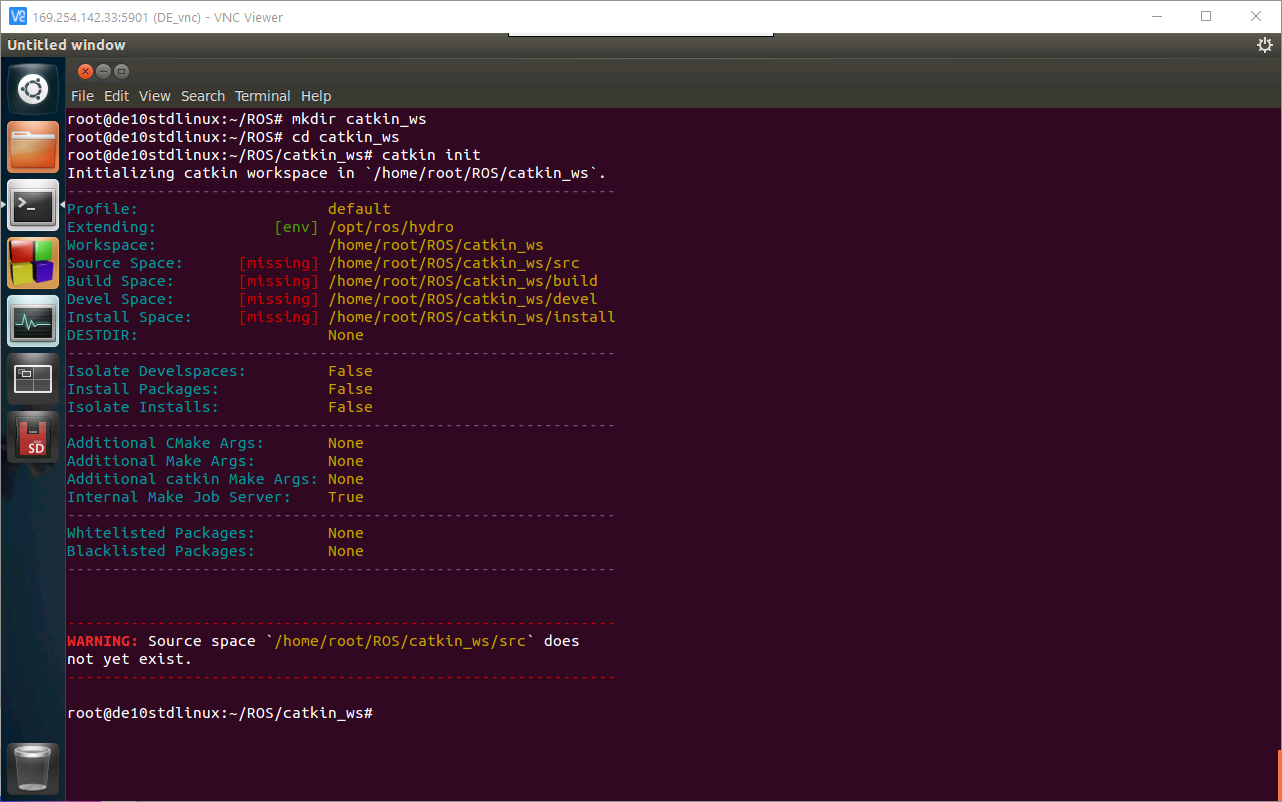
\includegraphics[scale=0.55]{figures/create_catkin_ws.png}
		\caption{Creation of a Catkin Workspace - Part I}
		\label{fig:createcatkinws}
	\end{center}
\end{figure}
\newpage
This creates and initializes a new catkin workspace in a new folder called {\sf catkin\_ws}. The newly created catkin workspace needs a source folder. Create a source folder using \lstinline|mkdir src| and then run \lstinline|catkin build| to have catkin automatically generate your workspace base. Notice that a build and a devel folder have automatically been created for you.
\begin{figure}[H]
	\begin{center}
		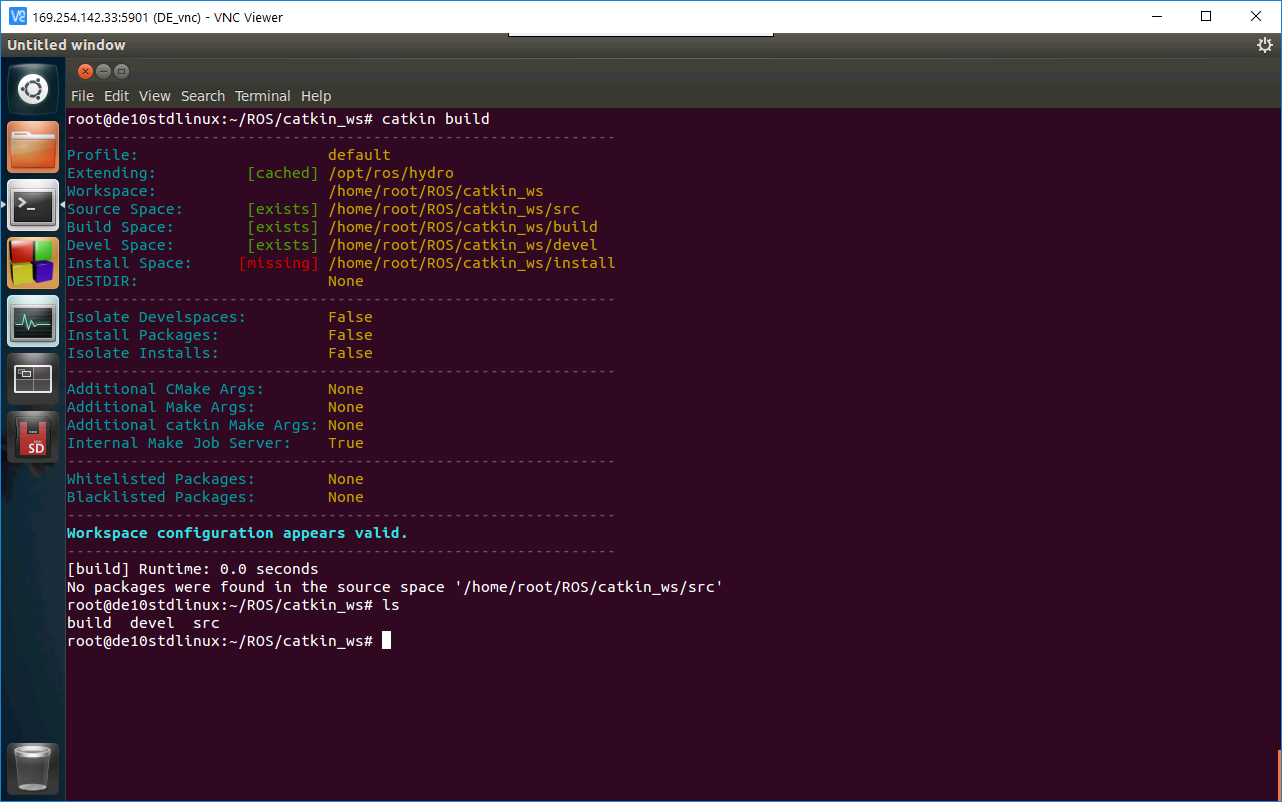
\includegraphics[scale=0.55]{figures/catkin_build_empty_ws.png}
		\caption{Creation of a Catkin Workspace - Part II}
		\label{fig:catkinbuildemptyws}
	\end{center}
\end{figure}
                    
\subsubsection{Creating a Package}
Under your first catkin workspace, you can create a catkin package by typing \lstinline|catkin create pkg --rosdistro HYDRO tutorial_pkg| in the source folder. This will create a default catkin package with the name {\sf tutorial\_pkg}.

We can build this package (which currently is empty) by again calling \lstinline|catkin build| in the root folder of this catkin workspace. By default this builds all packages in the \lstinline|src| folder and generates necessary environment variable information for the workspace. This environmental variable information can be brought into your current shell by running the command \lstinline|source devel/setup.bash| in the catkin workspace root. It is very important to source the setup.bash file after every build, or otherwise many ROS commands will not work properly.
\begin{figure}[H]
	\begin{center}
		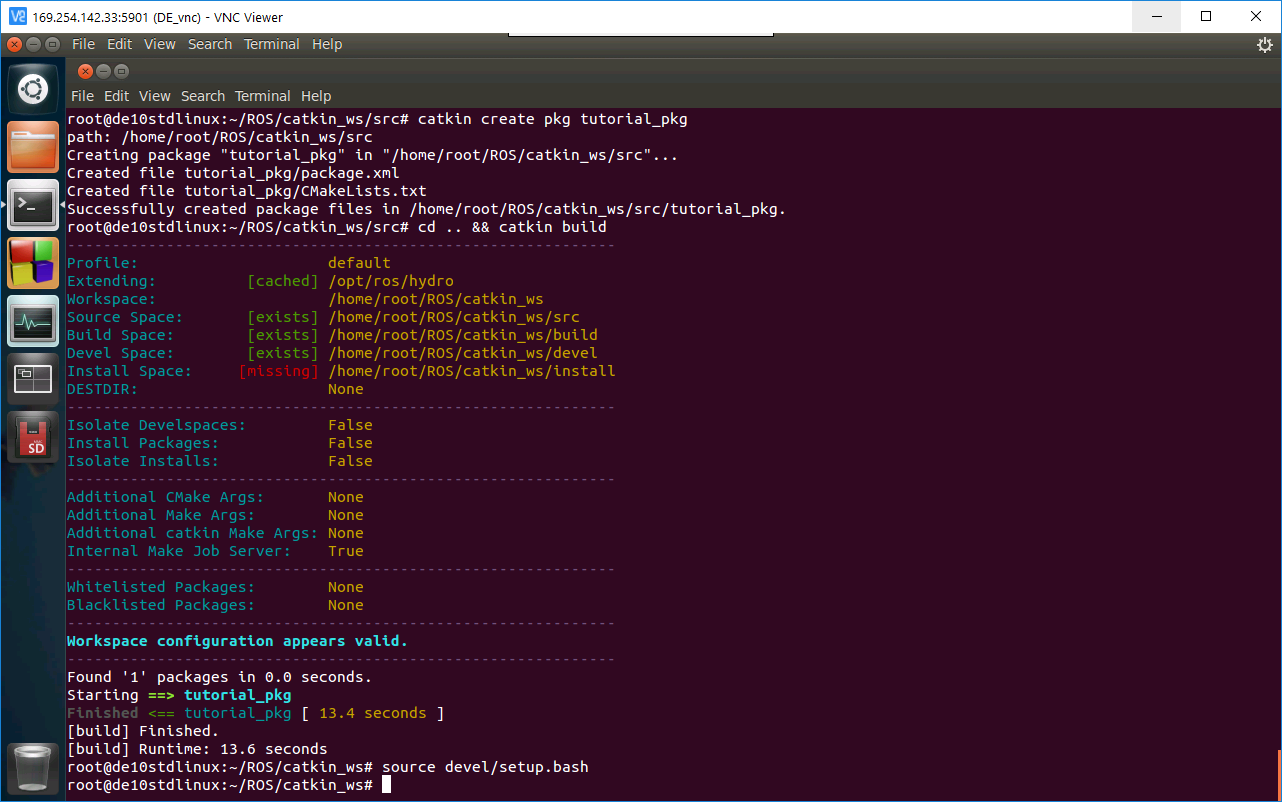
\includegraphics[scale=0.55]{figures/catkin_build_tutorial_pkg_1.png}
		\caption{Building your First Package}
		\label{fig:catkinbuildtutorialpkg1}
	\end{center}
\end{figure}

\section{Creating a Simple Publisher and Subscriber}
To add some functionality to our newly created package, we will create some ROS nodes. ROS nodes are essentially executables that are connected to the ROS network and serve as a basic building block of communications and data processing. Two of the most basic nodes of any ROS network are publisher and subscriber nodes. Publisher nodes distribute information to the ROS network by broadcasting a ROS message under a certain ROS topic name. Subscriber nodes can then subscribe to the ROS topic to read the information that the publisher node has published.

\subsection{Creating a Publisher}
We want to create a publisher node in our {\sf tutorial\_package}. Lets begin by changing to the directory that our package is contained in and creating a .cpp file for our code.
\begin{lstlisting}
roscd tutorial_pkg/
mkdir src
touch src/tutorial_publisher.cpp
\end{lstlisting}
Next, open up the file in a text editor of your choice and insert the following code:
\begin{figure}[H]
\begin{lstlisting}
#include <ros/ros.h>
#include <std_msgs/UInt16.h>

void publishData(ros::Publisher pub)
{
	std_msgs::UInt16 msg;
	msg.data = 1;
	pub.publish(msg);
	ROS_INFO("Published: %d", msg.data);
}

int main(int argc, char** argv)
{
	ros::init(argc, argv, "publisher");
	ros::NodeHandle nh;
	ros::Publisher pub = nh.advertise<std_msgs::UInt16>("published_data", 100);
	
	ros::Rate loop_rate(10); // 10Hz
	while(ros::ok())
	{
		publishData(pub);
		loop_rate.sleep();
	}
}
\end{lstlisting}
\caption{Code for the publisher}
\end{figure}
The code above creates a very simple publisher that creates to the topic "published\_data" on the ROS network and publishes data to the topic using the \lstinline|publishData()| function. There are three major sections to the code:
\begin{enumerate}
	\item In lines 4-10, we define the \lstinline|publishData()| function. This function publishes the number 1 using the publisher it gets passed in as an argument. Lines 6-7 create a \lstinline|std_msgs::UInt16| message and set its data to the number 1. Line 8 publishes the created message, and line 9 calls \lstinline|ROS_INFO()| which prints a message to the console that indicates a successful publishing of the message.
	\item In lines 14-16, we initialize the ROS node. Line 14 initializes the ROS framework using the command \lstinline|ros::init()| which gets passed \lstinline|argc|,~\lstinline|argv| and the name of the node to be created. Line 15 instantiates the \lstinline|ros::NodeHandle| object, which is used as an access point for all communications objects in ROS. Line 16 then uses the \lstinline|NodeHandle| object to create a \lstinline|ros::Publisher| that publishes to the ROS topic "published\_data" with a buffer of 100.
	\item In lines 18-23, we do the actual work of the node. Line 18 and line 22 together create and use a \lstinline|ros::Rate| object to ensure that the \lstinline|while| loop runs at a frequency of 10 Hz. Each time the \lstinline|while| loop is called, it first checks \lstinline|ros::ok()| in line 19, which returns \lstinline|false| only if a SIGINT is received, this node is somehow shut down, the ROS network is somehow shut down, or no  NodeHandle objects exist. Finally, in line 21 we call the function which will publish the desired data.
\end{enumerate}

\subsection{Creating a Subscriber}
Next, we want to create a subscriber node in our {\sf tutorial\_package}. Go back to our package is contained in and create a .cpp file for our code.
\begin{lstlisting}
roscd tutorial_pkg/
touch src/tutorial_subscriber.cpp
\end{lstlisting}
Open up the file in a text editor of your choice and insert the following code:
\begin{figure}[H]
\begin{lstlisting}
#include <ros/ros.h>
#include <std_msgs/UInt16.h>

void subCallback(const std_msgs::UInt16 msg)
{
	ROS_INFO("Message reads: %d", msg.data);
}

int main(int argc, char** argv)
{
	ros::init(argc, argv, "subscriber");
	ros::NodeHandle nh;
	ros::Subscriber sub = nh.subscribe<std_msgs::UInt16>("published_data", 100, subCallback);
	
	ros::Rate loop_rate(10); // 10Hz
	while(ros::ok())
	{
		ros::spinOnce();
		loop_rate.sleep();
	}
}
\end{lstlisting}
\caption{Code for the subscriber}
\end{figure}
The code above creates a very simple subscriber that connects to the topic "published\_data" on the ROS network and reads and processes data via the subCallback() function. Again, there are three major sections to the code:
\begin{enumerate}
	\item Lines 4-7 define the subCallback() function that processes messages incoming into the subscriber node. Currently, we just print the data contained in the message to the console in line 6 with a \lstinline|ROS_INFO()| call.
	\item Lines 11-13 function much the same as in the publisher node in that we are creating and initializing the ROS node. The major difference here is that in line 11 we are creating a \lstinline|ros::Subscriber|, which has an additional third parameter that we must pass to it to designate the callback function that is called when the subscriber gets a message. Here, we pass it the \lstinline|subCallback()| function. Note that the signal parameter of the callback function gets automatically assigned to a pointer to the incoming ROS message when it is called by the \lstinline|ros::Subscriber| object.
	\item Lines 15-20 do the actual work of the node. Here, we again set a loop rate to run the node at 10 Hz, but instead of calling a publishing function in the \lstinline|while| loop as we did in the publisher, we instead call \lstinline|ros::spinOnce()|. This function tells the ROS node to go through all the messages that its \lstinline|ros::Subscriber| objects have received and call the corresponding callback function for each one. Without this function call, our node would just keep recording messages on the topic \lstinline|published_data| into a queue but never actually do anything!
\end{enumerate}

\subsection{Configuring Cmake}
Catkin uses cmake to manage, build, and install packages. When you created a package in the previous section, the package automatically comes with a CMakeLists.txt that tells cmake what to do with the package during the build process. Additionally, because the package was created using python-catkin-tools, the CMakeLists.txt file comes with some commented out lines that serve as a basic guide for configuring cmake.

Now that we have finished writing the code for our publisher and subscriber, we must get the catkin workspace to build the publisher with our project. Open up the CMakeLists.txt file in the tutorial package directory and navigate to the line that contains the \lstinline|find_package()| call. This command locates packages and sets cmake variables depending on if it was able to successfully locate those packages. In ROS, this is typically used to specify that your package depends on certain other packages given by this command. For this tutorial, we need to change the line to the following:
\begin{lstlisting}
	find_package(catkin REQUIRED COMPONENTS roscpp std_msgs)
\end{lstlisting}

Next, navigate to the line that contains the \lstinline|add_executable()| call. This command adds a target to be built by cmake. The first parameter is the name of the target, and the second parameter is the location of the source file to be built. For our package, we have two targets: the publisher and the subscriber, so we need to modify the lines as follows:
\begin{lstlisting}
	add_executable(publisher src/tutorial_publisher.cpp)
	add_executable(subscriber src/tutorial_subscriber.cpp)
\end{lstlisting}

Then, navigate to the line that contains the \lstinline|add_dependencies| call that is located after the \lstinline|add_executable()| calls we just added. This command tells cmake what your targets depend to determine the workspace build order. Here, we need to depend on \lstinline|${catkin_EXPORTED_TARGETS}| which tells cmake to build all message or service headers before building any of our targets. For our package, we use \lstinline|std_msgs| and so require that to be built first. Therefore, lets add the following lines:
\begin{lstlisting}
	add_dependencies(publisher ${catkin_EXPORTED_TARGETS})
	add_dependencies(subscriber ${catkin_EXPORTED_TARGETS})
\end{lstlisting}

Finally, navigate to the line that contains the \lstinline|target_link_libraries()| call. This command tells cmake which libraries the linker should link our targets against. For now, we only need to link against \lstinline|${catkin_LIBRARIES}|, and so we should change the lines to the following:
\begin{lstlisting}
	target_link_libraries(publisher
		${catkin_LIBRARIES}
	)
	target_link_libraries(subscriber
		${catkin_LIBRARIES}
	)
\end{lstlisting}
There are many other catkin configuration parameters that will be useful and necessary in building certain other projects. We recommend the user to reference the ROS hydro catkin documentation located at \url{docs.ros.org/hydro/api/catkin/html/index.html} for more information on configuring cmake with catkin.

\subsection{Configuring your Package Manifest}
You may have noticed that along with creating a CMakeLists.txt, the call to \lstinline|catkin create pkg| also created a package.xml file. This is a file that contains information about our package properties, including meta-data such as package name, author, etc. as well as dependency information on other packages. For the tutorial package, we only depend on the \lstinline|std_msgs| ROS package, and so we need to add the following lines to our package.xml:
\begin{lstlisting}
	<depend>std_msgs</depend>
\end{lstlisting}
Depending on what you do with your package and the contents inside, your package.xml may be much more complicated than in this example. It is highly recommended to browse the ROS wiki's package.xml page located at \url{http://wiki.ros.org/catkin/package.xml} for more information on writing the package.xml file.

\subsection{Running Your First ROS Node}\label{sec:rosrun}
Now that the build process of the tutorial package is properly configured, we can compile the project and run each ROS node. Change directories back to the root of our catkin workspace, build the catkin packages, and source the workspace. Because we actually have some code to build this time, the processor may take some time to process the commands.
\begin{lstlisting}
	cd ~/ROS/catkin_ws
	catkin build
	source devel/setup.bash
\end{lstlisting}

\begin{figure}[H]
	\begin{center}
		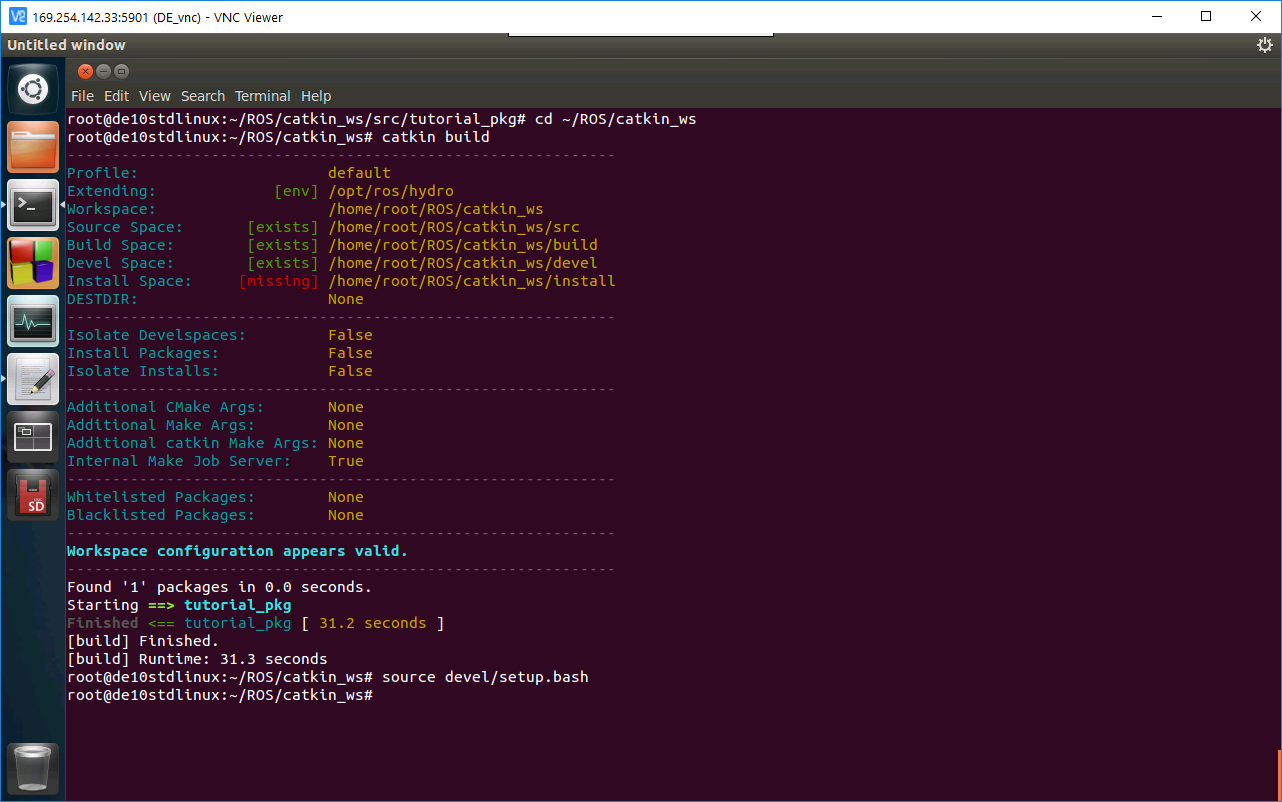
\includegraphics[scale=0.55]{figures/catkin_build_tutorial_pkg_2.png}
		\caption{Building the Semi-complete Package}
		\label{fig:catkinbuildtutorialpkg2}
	\end{center}
\end{figure}

After the build finishes, open up three new terminals. In each terminal, first source the setup.bash file in our catkin workspace 
\begin{lstlisting}
	cd ~/ROS/catkin_ws
	source devel/setup.bash
\end{lstlisting}
Then in the first terminal, run \lstinline|roscore|. \lstinline|roscore| is a set of ROS nodes that facilitate the base functionalities of the ROS network. You can think of this as "turning on" the ROS network. Additionally, \lstinline|roscore| must be run before starting any other nodes, and failure to do so will result in an error during the initialization of your node.

In the second terminal, run \lstinline|rosrun tutorial_pkg publisher|. This starts the ROS node that we wrote to publish information to the \lstinline|published_data| topic. You should see the \lstinline|ROS_INFO| printouts of the timestamp and published message.

In the third terminal, run \lstinline|rosrun tutorial_pkg subscriber|. This starts the ROS node that we wrote to subscribe to the \lstinline|published_data| topic. You should see the \lstinline|ROS_INFO| printouts of the timestamp and received message. Note that the received message is the same as the published message, but there is a difference in the timestamps that indicate the delay between sending and receiving the message.

\begin{figure}[H]
	\begin{center}
		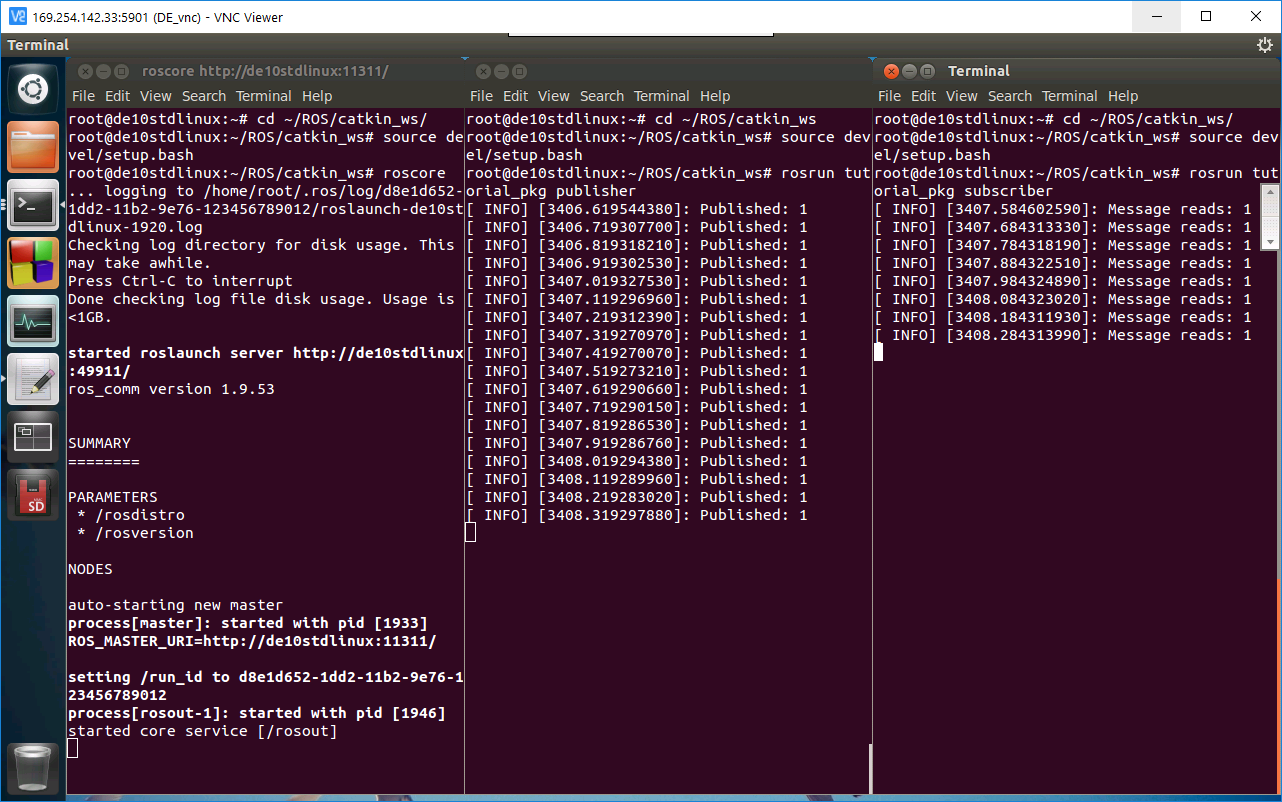
\includegraphics[scale=0.55]{figures/rosrun_tutorial_pkg_1.png}
		\caption{Running the Tutorial Package}
		\label{fig:rosruntutorialpkg1}
	\end{center}
\end{figure}

Once you are satisfied with the results, hit ctrl-C on each of the terminals to stop the ROS commands being run.

\section{Interacting with Hardware Components}
Now lets add some functionality to the publisher and subscriber. Our overall goal will be to create a system that allows us to control the LEDs by using the switches on the DE-Series board. Our simple ROS system will consist of a publisher that constantly polls the state of the switches. The state of the switches will be represented by a binary number where the ith digit of the binary number being 1 represents the ith switch being toggled in the on state. The publisher will broadcast this binary number in an \lstinline|uint16| variable, which will then be packaged into a message that in broadcasted onto the ROS network under the topic \lstinline|/published_data|. On the other hand, our subscriber will be actively monitoring this ROS topic and set the LED lights based on the information in the messages it sees on the ROS topic. 

\newpage
\subsection{Accessing the Prebuilt Device Drivers}
To access the switches and LED hardware components, we need to use the prebuilt libraries for hardware access that are included in the Linux image. These libraries are located at \lstinline|~/Linux_Libraries/C4DE/include|. To use these libraries with our project, we must include the header files in the C++ source code, tell CMake to link the intelfpgaup.so library when building the project, and make sure to insert corresponding kernel modules during runtime. For the first step, we add the lines in Figures \ref{lst:publisherheader} and \ref{lst:subscriberheader} below to the beginning of tutorial\_publisher.cpp and tutorial\_subscriber.cpp respectively. Note that the libraries used to access the hardware components are built in C, while ROS runs on C++. This means that we must add the linkage-specification \lstinline|extern "C"| and the pre-processor directive \lstinline|#ifdef __cplusplus| when we include the header files to specify that these are C header files being used in C++ (for more information on why this is necessary, feel free to search up “name mangling” on the Internet). 

{\it Note: on the DE10-Nano, the LEDR driver and its corresponding wrappers are named LED. For the DE0-Nano, please reference the files at \lstinline|~/Linux_Libraries/C4DE/include| for header name changes. Make sure to change the code in this section accordingly to match your board.}

\begin{figure}[H]
\begin{lstlisting}
	#ifdef __cplusplus
	extern "C" {
	#endif
	#include <intelfpgaup/SW.h>
	#ifdef __cplusplus
	}
	#endif
\end{lstlisting}
\caption{Header include for publisher}
\label{lst:publisherheader}
\end{figure}

\begin{figure}[H]
	\begin{lstlisting}
	#ifdef __cplusplus
	extern "C" {
	#endif
	#include <intelfpgaup/LEDR.h>
	#ifdef __cplusplus
	}
	#endif
	\end{lstlisting}
	\caption{Header include for subscriber}
	\label{lst:subscriberheader}
\end{figure}
Next, to link the intelfpgaup.so library, we first need to let cmake know where our library is located. Open up the CMakeLists.txt file that is in the root folder of our package and add the following line right after the \lstinline|catkin_package()| call.
\begin{lstlisting}
find_library(intelfpgaup_LIBRARIES NAMES libintelfpgaup.so PATHS /root/home/Linux_Libraries/C4DE)
\end{lstlisting}
The above call to \lstinline|find_library()| tells cmake to look in a specified path for our intelfpgaup.so library and assign the cmake variable \lstinline|intelfpgaup_LIBRARIES| accordingly. Now, to specify that we want to link these libraries to the target, we add the generated cmake variable to our \lstinline|target_link_libraries()| call for both our publisher and subscriber nodes. In the end, it should look something like this:
\begin{lstlisting}
	target_link_libraries(publisher
		${catkin_LIBRARIES}
		${intelfpgaup_LIBRARIES}
	)
	target_link_libraries(subscriber
		${catkin_LIBRARIES}
		${intelfpgaup_LIBRARIES}
	)
\end{lstlisting}
Note that while we must individually include the library header file for each hardware component that we are using (eg. LEDR.h), we only have to link the intelfpgaup.so library once to each target in the CMakeLists.txt file. 

Finally, to insert the kernel modules for each file, simply run the command \lstinline|insmod <path-to-module>| where <path-to-module> points to one of the kernel modules found in the folder \lstinline|~/Linux_Libraries/drivers|. For this tutorial, we will need to insert the switches.ko and LEDR.ko modules.

\begin{figure}[H]
	\begin{center}
		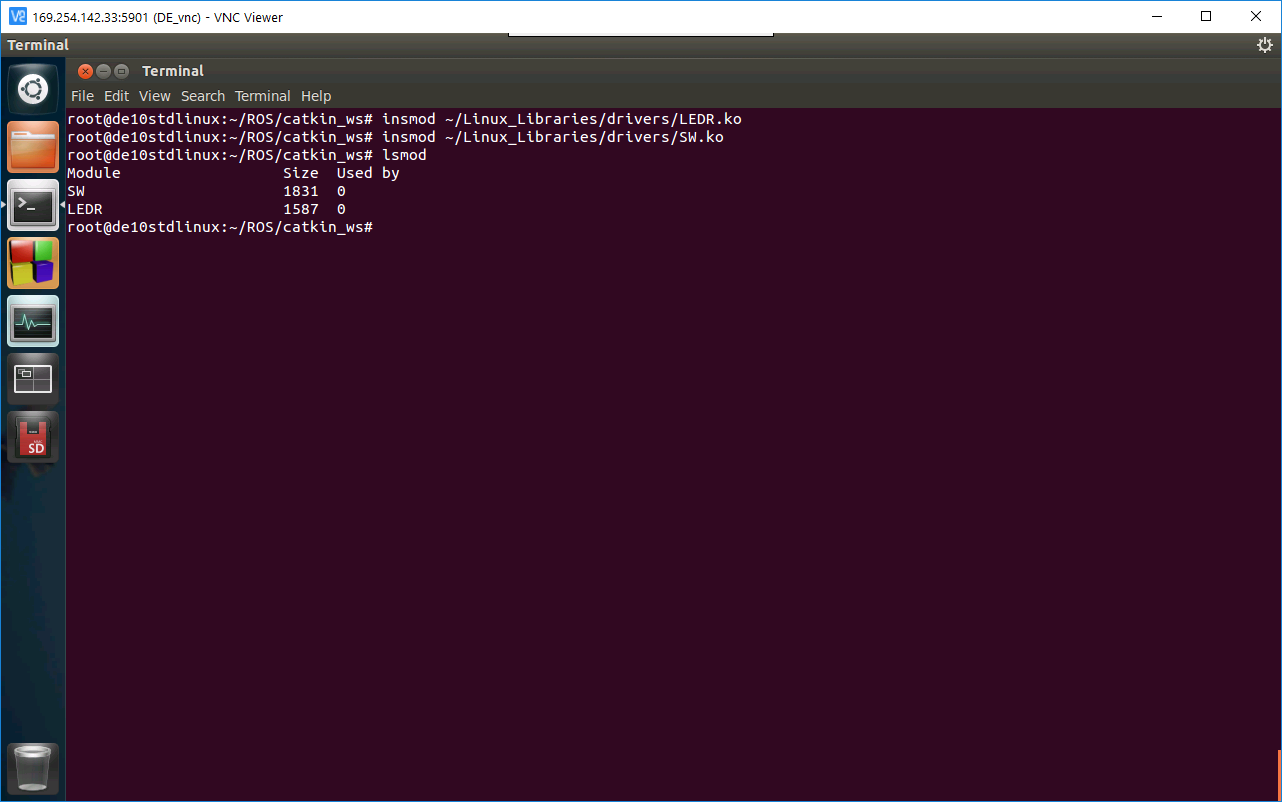
\includegraphics[scale=0.55]{figures/insmod_SW_LEDR.png}
		\caption{Inserting the Kernel Modules}
		\label{fig:insmodSWLEDR}
	\end{center}
\end{figure}

\newpage
\subsection{Using the Prebuilt Device Drivers}
Now, lets update the contents of our publisher and subscriber. Modify the code of tutorial\_publisher.cpp and tutorial\_subscriber.cpp to match the code shown in the corresponding figures below.

\begin{figure}[H]
	\begin{lstlisting}
	#include <ros/ros.h>
	#include <std_msgs/UInt16.h>
	
	#ifdef __cplusplus
	extern "C" {
	#endif
	#include <intelfpgaup/SW.h>
	#ifdef __cplusplus
	}
	#endif
	
	void publishData(ros::Publisher pub) 
	{
		std_msgs::UInt16 msg;
		int data;
		if(SW_read(&data))
		{
			msg.data = data;
			pub.publish(msg);
		}
	}
	
	int main(int argc, char** argv)
	{
		ros::init(argc, argv, "publisher");
		ros::NodeHandle nh;
		ros::Publisher pub = nh.advertise<std_msgs::UInt16>("published_data", 100);
		
		ros::Rate loop_rate(10);
		if(SW_open() != 1) return -1;
		while(ros::ok())
		{
			publishData(pub);
			loop_rate.sleep();
		}
		SW_close();
	}
	\end{lstlisting}
	\caption{Code for the Publisher}
	\label{lst:publishData()}
\end{figure}
\begin{figure}[H]
	\begin{lstlisting}
	#include <ros/ros.h>
	#include <std_msgs/UInt16.h>
	
	#ifdef __cplusplus
	extern "C" {
	#endif
	#include <intelfpgaup/LEDR.h>
	#ifdef __cplusplus
	}
	#endif
	
	void switchCallback(const std_msgs::UInt16::ConstPtr& msg)
	{
		LEDR_set(msg->data);
	}
	
	int main(int argc, char** argv)
	{
		ros::init(argc, argv, "subscriber");
		ros::NodeHandle nh;
		ros::Subscriber sub = nh.subscribe<std_msgs::UInt16>("published_data", 100, switchCallback);
		
		ros::Rate loop_rate(10);
		if(LEDR_open() != 1) return -1;
		while(ros::ok())
		{
			ros::spinOnce();
			loop_rate.sleep();
		}
		LEDR_close();
	}
	\end{lstlisting}
	\caption{Code for the Subscriber}
	\label{lst:switchCallback()}
\end{figure}

The usage of the intelfpgaup.so library for hardware component access is fairly straightforward, and a copy of the header files with documentation can be found in Appendix D of this document. Briefly, each hardware component is controlled by first opening a connection to the hardware component using the \lstinline|open()| command. Then, we can read or write using the specific functions included in the header file for that hardware component. For example, in line 16 of Figure \ref{lst:publishData()} we read from the switches port by calling the \lstinline|SW_read()| function provided by the switches.h header file. Similarly, we write to the LEDR hardware component by calling the \lstinline|LEDR_set()| function in line 14 of Figure \ref{lst:switchCallback()}. Finally, when we are done using the hardware components, we must make sure to close the connection to them using the \lstinline|close()| command, as seen in line 36 of Figure \ref{lst:publishData()} and line 30 of Figure \ref{lst:switchCallback()}.

\subsection{Testing the Tutorial Package}
With all the code set, we can once again try running our package. In a new terminal window, change directories to the root of your catkin workspace and run the following commands  
\begin{lstlisting}
	catkin clean --build
	catkin build
	source devel/setup.bash
	roscore &
	rosrun tutorial_pkg publisher &
	rosrun tutorial_pkg subscriber &
\end{lstlisting}
This starts the three ROS processes mentioned in Section \ref{sec:rosrun} in a single terminal (which is useful for not cluttering up your screen). To make sure that the nodes are working correctly, you can open up a new terminal window, source the setup.bash file in your catkin workspace, and run \lstinline|rostopic echo /published_data|. This  echos the messages being published to \lstinline|/published_data| in your terminal. Try flipping some of the switches and seeing if the published messages change accordingly. You should see an output similar to the image in Figure \ref{fig:rosruntutorialpkg2}, and be able to observe the LEDs on your DE-Series board changing according to the position of the switches. 

\begin{figure}[H]
	\begin{center}
		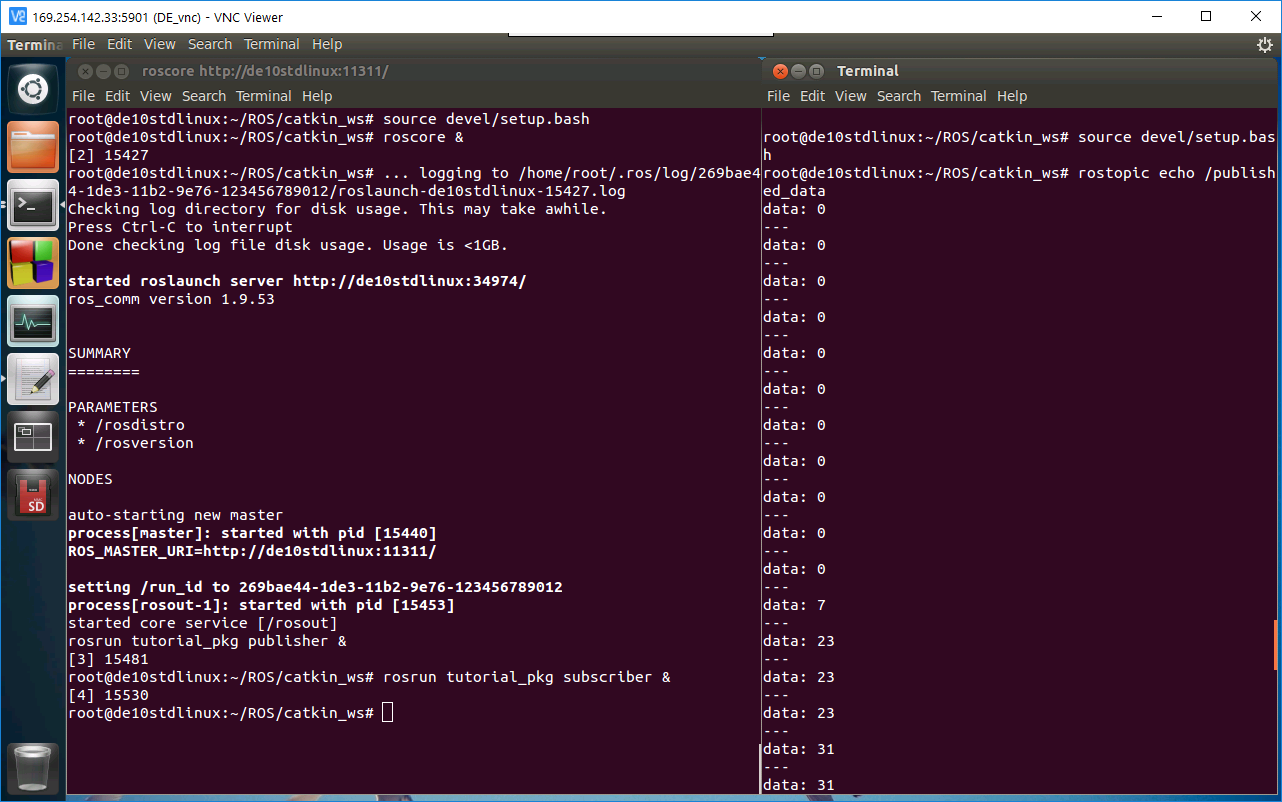
\includegraphics[scale=0.55]{figures/rosrun_tutorial_pkg_2.png}
		\caption{Running the Tutorial Package with Hardware Interaction}
		\label{fig:rosruntutorialpkg2}
	\end{center}
\end{figure}
Once you are satisfied with the results, close the terminal window to terminate the ROS processes.
\subsection{Using Custom Hardware with ROS}
It is also possible to interact with custom hardware connected to the DE-Series board. While the interaction with ROS would be done in a similar way as described above, the user must also write a custom driver to access the hardware. Detailed instructions for writing custom drivers for the DE-Series boards can be found in the tutorial {\it Linux on DE Series Boards} under the section {\it Device Drivers}. This tutorial is located on the Intel FPGA University Program Website.


\newpage
\section*{Appendix A~~~~ Using Intel\textsuperscript{\textregistered} FPGA Device Drivers}

\noindent In addition to being able to create your own kernel modules, as 
discussed above, the \textit{DE1-SoC-UP} Linux distribution provides a number of pre-built
kernel modules that are available for communicating with hardware modules in the DE1-SoC 
Computer. These pre-built modules are listed in Table 1.

Each of the kernel modules listed in Table 1 provides a {\it character device driver} for
accessing a port in the DE1-SoC Computer. This means that each module has a file-based
interface that can be used to read information from the driver, or write information to
it. The file-based interface is provided in the folder \texttt{/dev/IntelFPGAUP}. One way to
read from a driver is to use the Linux \texttt{cat} command. For example, to read the
states of the pushbutton switches you can type \texttt{cat /dev/IntelFPGAUP/KEY}. Usage 
information for each driver can be found by writing \texttt{-$\,$-} to the driver. For example, 
to see how to use the video driver you could type the Linux command
\texttt{echo -$\,$- > /dev/IntelFPGAUP/video}. 

The drivers listed in Table 1 are not inserted into the Linux kernel during the boot
process. To insert a driver, navigate to the directory
\texttt{/home/root/Linux\_Libraries/drivers}. To insert a specific driver, you can use the
Linux command \texttt{insmod}. For example to insert the \texttt{KEY} driver you would
type \texttt{insmod KEY.ko}. To insert all available drivers, you can execute the script
\texttt{load\_drivers}. Similarly, you can then remove an individual driver by using the
command \texttt{rmmod}, or remove all of the drivers by executing the script
\texttt{remove\_drivers}.

For convenience, a set of {\it wrapper} functions is provided in the C language for use with 
each character device driver. To use these functions in a program, you need 
to provide the statement \texttt{\#include "IntelFPGAUP/{\it xxx}.h"} in your C code, 
where {\it xxx} is the name of the driver from Table 1 (\texttt{KEY}, \texttt{SW}, $\ldots$). 
In addition, you have to append the option \texttt{-lintelfpgaup} to the \texttt{gcc} command when 
compiling your code. The contents of the files {\it xxx.h}, which list all of the 
available wrapper functions, are shown in Appendix B. The wrapper source code
files and examples can be found in the directory \texttt{$\sim$/Linux\_Libraries/C4DE}.

\begin{table}[H]
\centering
\begin{tabular}{l|p{8cm}}
{\bf Kernel module}	&	{\bf Description}\\\hline
\rule{0cm}{.5cm}\texttt{KEY}	&	Used to access the pushbutton KEY port\\
\texttt{SW}		&	Used to access the slide switch SW port\\
\texttt{LEDR}	&	Used to access the red light LEDR port\\
\texttt{HEX}	&	Used to access the seven-segment HEX display port\\
\texttt{video}	&	Used to access the VGA video-out port\\
\texttt{audio}	&	Used to access the digital audio port\\
\texttt{accel}	&	Used to access the 3-D accelerometer port\\
\end{tabular}
\center{Table 1. Pre-built kernel modules}
\label{tab:drivers}
\end{table}

\subsubsection*{Drivers for the DE10-Standard Board}

If you are using the DE10-Standard board, then all of the device drivers listed in Table 1
are available, as well as their corresponding wrappers. In addition, there is a device
driver called \texttt{LCD}, which controls the $128 \times 64$ LCD display on the
DE10-Standard board. The wrappers provided for the \texttt{LCD} driver are identical to
those of the video driver in Table 1.

\subsubsection*{Drivers for the DE10-Nano Board}

If you are using the DE10-Nano board, then all of the device drivers listed in Table 1 are
available, except for the \texttt{HEX} driver. Also, for this board the \texttt{LEDR}
driver, and corresponding wrappers, is named \texttt{LED}.

\newpage
\section*{Appendix B~~~~ Wrapper Functions for using Character Device Drivers with C Code}

\subsection*{Header File for Pushbutton KEY Device}
\lstset{language=C,numbers=none}
\lstinputlisting{C4DE/include/KEY.h}
\newpage
\subsection*{Header File for Slide Switch SW Device}
\lstinputlisting{C4DE/include/SW.h}
\newpage
\subsection*{Header File for Red Light LEDR Device}
\lstinputlisting{C4DE/include/LEDR.h}
\newpage
\subsection*{Header File for Seven-Segment HEX Device}
\lstinputlisting{C4DE/include/HEX.h}
\newpage
\subsection*{Header File for VGA Video Device}
\lstinputlisting{C4DE/include/video.h}
\newpage
\subsection*{Header File for Digital Audio Device}
\lstinputlisting{C4DE/include/audio.h}
\newpage
\subsection*{Header File for 3-D Accelerometer Device}
\lstinputlisting{C4DE/include/accel.h}


% Copyright and Trademark

%\newcommand{\datePublished}{Mar 2022}

\newcommand{\versnum}{21.1} %version number quartus/AMP
\newcommand{\quartusname}{Quartus\textsuperscript{\textregistered} Prime}	
\newcommand{\textBar}{For \quartusname{} \versnum{}}
\newcommand{\thisyear}{2022 } %for copyright
\newcommand{\company}{FPGAcademy.org}
\newcommand{\longteamname}{FPGAcademy.org}
\newcommand{\teamname}{FPGAcademy}
\newcommand{\website}{FPGAcademy.org}

\newcommand{\productAcronym}{AMP}
\newcommand{\productNameShort}{Monitor Program}

\newcommand{\productNameMedTM}{Monitor Program}
\newcommand{\productNameMed}{Monitor Program}

%\newcommand{\headerLogoFilePath}[1]{#1/FPGAcademy.png}



%%%%%%%%%%%%%%%%%%%%%%%%%%%%%%%%%%%%%%%%
%%% FPGAcademy Copyright Information %%%
%%%%%%%%%%%%%%%%%%%%%%%%%%%%%%%%%%%%%%%%

%Always put the copyright on a new page (clear page), with some vertical space from top
\clearpage
\vspace{1in}

\noindent

Copyright {\copyright} FPGAcademy.org. All rights reserved. FPGAcademy and the FPGAcademy logo are trademarks of  FPGAcademy.org.  This document is being provided on an ``as-is'' basis and as an accommodation and therefore all warranties, representations or guarantees of any kind (whether express, implied or statutory) including, without limitation, warranties of merchantability, non-infringement, or fitness for a particular purpose, are specifically disclaimed.

%FPGAcademy assumes no responsibility or liability arising out of the application or use of any information,  product,  or  service  described  herein  except  as  expressly  agreed  to  in  writing  by  FPGAcademy.



**Other names and brands may be claimed as the property of others.




\end{document}

